\section*{Abstract}
We have developed and implemented a type system, the Signedness Type System,
that captures usage of signed and unsigned integers in Java programs. This
type system enables developers to detect errors regarding unsigned integers at
compile time, and guarantees that such errors cannot occur at run time. An
implementation of this type system for Java, the Signedness Checker, uncovered
previously unknown bugs in a case study. The Signedness Checker is available
publicly bundled with the Checker Framework (http://CheckerFramework.org/).

\newpage
\tableofcontents

\newpage
\section{Problem and Motivation}

Signed integers use the first bit of the machine representation to
encode the sign of a value, whereas unsigned integers use all
bits to represent the magnitude of a value.
As a result, unsigned integers can cover a larger range of nonnegative integer
values than signed integers given the same number of bits, but they are
incapable of representing negative integers. While signed integers are much
more common,
unsigned integers are also useful, so many programming languages support them;
for example, Java 8 introduced utility methods for unsigned
integers~\cite{JDK8UnsignedIntegerArithmetic2012}.  However, they are also
error-prone:  using one where a signed
integer is expected, or performing certain arithmetic operations on unsigned
integers, can lead to unexpected results.

For the duration of this paper,
we call an operator ``insensitive'' if it produces a correct signed result
when run on two signed values and a correct unsigned result
when run on two unsigned values.  We call an operator ``sensitive'' if it
produces incorrect results when run on two unsigned values. For such
operations, a programmer must run a different implementation depending on
whether
the operands are signed or unsigned.
See Figure~\ref{fig:operators} for
an example of insensitive and sensitive operators.

\begin{figure}[t]
\begin{lstlisting}
\\ Signed: -3, Unsigned: 253
byte a = 0xFFFD;

\\ Signed: 2, Unsigned: 2
byte b = 0x0002;

\\ - is an insensitive operator and thus either
\\ interpretation is consistent
\\ Signed: -1, Unsigned: 255
byte sum = a - b;

\\ / is a sensitive operator and thus only the
\\ operator interpretation is always consistent
\\ (in this case signed)
\\ Signed: -1, Unsigned: 255 (expected 126)
byte div = a / b;
\end{lstlisting}
\vspace{-10pt}
\caption{An example of the distinction between insensitive and sensitive
operators.}
\label{fig:operators}
\end{figure}

Misuse of unsigned values can be categorized as follows:

\begin{itemize}\itemsep 0pt \parskip 0pt
  \item Using a sensitive operator with unsigned operands.
  \item Mixing signed and unsigned arguments to any operator.
\end{itemize}

See Figure~\ref{fig:misuse} for
an example of misuses of unsigned values.

\begin{figure}[t]
\begin{lstlisting}
\\ Using unsigned integers in a sensitive operator
\\ can lead to incorrect results
\\ Unsigned: 255
byte a = 0xFF;

\Unsigned: 254
byte b = 0xFE;

\Unsigned: 0 (expected 1)
byte div = a / b;

\\ Mixing signed and unsigned integers leads to
\\ incomprehensible results
\\ Signed: 1
byte s = 0x01;

\\ Unsigned: 127
byte u = 0x7F;

\\ Signed: -128, Unsigned: 128
byte sum = s + u;

\\ How do we even interpret this?
\\ Do we print -128 or 128?
System.out.println(sum);
\end{lstlisting}
\vspace{-10pt}
\caption{An example of possible misuses of unsigned integers.}
\label{fig:misuse}
\end{figure}

The first line of defense against most bugs is the compiler. When the
compiler is unable to catch bugs, it falls on the programmer to identify and
eliminate them, which is prone to human error. The Java compiler
is not helpful in finding bugs related to using unsigned
numbers because Java's unsigned
integers are supported by a library rather than built into the core language.

\section{Approach and Uniqueness}

\subsection{Core Design}

Our approach to detecting and preventing signedness errors is to use a type
system. This has a number of benefits. Firstly, compile-time checking permits
developers
to catch bugs before they become problems for end-users. Secondly, static
checking provides a guarantee across all program executions.
Finally, type systems are familiar to programmers,
who understand how to use them
and interpret their warning messages.

\begin{figure}[t]
    \centering
    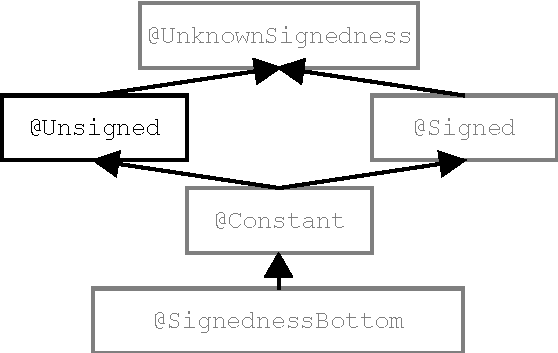
\includegraphics{signedness}
    \vspace{-10pt}
    \caption{The type qualifier hierarchy of our type system.
    Qualifiers in gray are used internally, and should not be written.}
    \label{fig:type-hierarchy}
\end{figure}

We have defined a type system and implemented it in a tool
called the Signedness Checker.
This type system has five type qualifiers
(Figure~\ref{fig:type-hierarchy}).  Each is written together
with a base type; for example, \<@Unsigned int i> declares a
variable named \<i> of type \<@Unsigned int>. The specific semantics of
each qualifier in the system follows:

\begin{itemize}\itemsep 0pt \parskip 0pt
  \item \<@UnknownSignedness> indicates a value for which our tool
   has no estimate.  (This usually leads to a
    warning.)  It is also used for non-numeric
    values, which our tool ignores.
  \item \<@Unsigned> signifies that a value is unsigned.
  \item \<@Signed> signifies that a value is signed.
  \item \<@Constant> is for values known at compile time, such as
    manifest literals.  The programmer might intend to
    use them as signed or as unsigned values.  Even a negative literal may
    be used as a placeholder for a large positive unsigned
    integer.
  \item \<@SignednessBottom> indicates dead code or the \<null> value.
\end{itemize}

The programmer writes \<@Unsigned> type qualifiers on type uses
in the program's source code.  Unannotated Java types
are given a default qualifier. Our systems type introduction rules follow:

\begin{enumerate}\itemsep 0pt \parskip 0pt
  \item If the user wrote a type qualifier, use it.
  \item If an integral expression is a constant at compile time, use
    \<@Constant>.
    Integral types are \<char>, \<byte>, \<short>, \<int>, \<long>, \<Integer>, and \<Long>.
  \item Other integral expressions use \<@Signed>.
  \item Binary integral operators have the least upper bound of the types of
  its operands as its type.
  \item Non-integral expressions use \<@UnknownSignedness>.
\end{enumerate}

The type rules of the Signedness Type System issue a warning if a program
might perform a computation using operands of incorrect or mixed signedness.
These type rules are as follows:

\begin{itemize}\itemsep 0pt \parskip 0pt
  \item Unsigned values may not be used with sensitive
    operators.
  \item With the exception of shifts, no operator may operate on a mix of
    signed and unsigned values.
  \item Logical right shifts may only be applied to unsigned values.
  \item Arithmetic right shifts may only be applied to signed values.
\end{itemize}

\subsection{Incremental Improvements}

As stated, the Signedness Type System cannot precisely analyze shift
expressions. Specifically, it may identify errors incorrectly in three cases:

\begin{enumerate}
  \item The type system does not correctly propogate a shift expression's type.
  \item A shift expression is masked by some literal which renders the
  signedness of the shift irrelevent to the mask's result.
  \item A shift expression is casted down such that the signedness of the
  shift is irrelevent to the casted result.
\end{enumerate}


\subsubsection{Shift Propogation}
We recall that the type of most binary operators is the least upper bound of
the types of its operands.
However, in the case of shifts, this is imprecise.
The reason for this is that shifts are applied to the left operand, using the
right operand to dictate how the shift is applied. Additionally, the bounds
set by Java on the allowable values for the right operand keep its true value
well within the signed positive range. This means that only the signedness
of the left operand of a shift expression is relevant to its signedness.
Therefore, the type of a shift expression is the type of its left operand. See
Figure~\ref{fig:shiftpropo} for an example of false errors issue by the
Signedness Type System without this change.

\begin{figure}[t]
\begin{lstlisting}
//TODO FIND CODE
\end{lstlisting}
\vspace{-10pt}
\caption{An example of code for which the Signedness Checker will issue a false
alarm due to shift propogation.}
\label{fig:shiftpropo}
\end{figure}

\subsubsection{Masked Shifts}
We recall that the type rule for right shifts is that the signedness of the left
operand must match the signedness of the shift. However, when the result of the
shift is masked by certain values, the introduced bits are discarded and the
signedness of the shift becomes irrelevent. See Figure~\ref{fig:maskedshift}
for an example of this situation. To solve this problem, we check if every
right shift is nested in a mask. If it is, we then compare the shift value
and mask literal to see if the bits introduced by the shift are masked away.
If they are, then we issue no error. Otherwise, we refer back to the previous
behavior.

\begin{figure}[t]
\begin{lstlisting}
// The Signedness Checker issues 3 warnings because
// unsigned right shift changes its argument's sign
// by filling in zeroes in the most significant bits.
// This doesn't matter in the below code snippet,
// because all of the introduced bits are masked off.

@Signed int c;
sb.data[i++] = (byte) ((c >>> 8) & 0xff);
sb.data[i++] = (byte) ((c >>> 16) & 0xff);
sb.data[i++] = (byte) ((c >>> 24) & 0xff);

\end{lstlisting}
\vspace{-10pt}
\caption{An example of code for which the Signedness Checker will issue a false
alarm due to masked shifts, from our case study of jake2.}
\label{fig:maskedshift}
\end{figure}

\subsubsection{Casted Shifts}
We recall again that the type rule for right shifts is that the signedness
of the left
operand must match the signedness of the shift. However, when the result of the
shift is casted down to certain types, it could be the case that the bits
introduced by the shift are discarded by the cast, rendering the signedness of
the shift irrelevent to the result of the cast.
See Figure~\ref{fig:castedshift} for an example of this situation. To solve this
problem, we check if every right shift is nested in a cast. We then compare the
shift value and the type of the shifted value to the type of the cast target
to see if the introduced bits are discarded or not. If they are then we do not
issue an error. If not, then we defer to the prevous behavior.

\begin{figure}[t]
\begin{lstlisting}
//TODO FIND CODE
\end{lstlisting}
\vspace{-10pt}
\caption{An example of code for which the Signedness Checker will issue a false
alarm due to casted shifts.}
\label{fig:castedshift}
\end{figure}

\section{Background and Implementation}

Our goal is to build a verification tool that guarantees that software is
free of bugs related to unsigned integers. To achieve this, our approach
must be sound:  if it issues no warnings, then the program must be free of
bugs.
Any sound analysis sometimes issues false positives --- warnings about
code that will not go wrong at run time.  This occurs when the
Signedness Checker cannot prove that the code is correct.

We built our Signedness Checker implementation upon the
Checker Framework~\cite{PapiACPE2008,DietlDEMS2011}, which enables the
construction of pluggable type systems for Java.
The Signedness Checker is distributed as part of the Checker Framework
(\url{http://CheckerFramework.org/}).

% For number of statements, count the number of semicolons, less those on
% lines starting with "package" or "import" or "//".
% Biggest component is by file size.
% The non-comment non-blank lines of code is about 300 for the type-checker
% plus about 100 for the type qualifiers (almost all of which are imports
% or meta-annotations).

Our pluggable type system implementation consists of fewer than 100
statements.  Its biggest component is a run-time library that provides
JDK~8 unsignedness functionality to earlier versions of Java.  The
type-checker consists of the following parts:

\begin{itemize}\itemsep 0pt \parskip 0pt
  \item Qualifiers are implemented as Java 8 type
    annotations~\cite{JSR308-PFD}.
  \item Type introduction rules are defined procedurally.
  \item Type rules are enforced by a traversal of the syntax tree.
\end{itemize}


\section{Results and Contributions}

We evaluated our tool by running it on jake2, a Java
port of the popular '90s video game, Quake II\@.  The original C
implementation of Quake II used unsigned integers. jake2
tries to mimic Quake II's usage and consists of 133513 lines of code that
can be found at (\url{https://github.com/mbien/jake2}).

TODO REST

\section{Related Work}

SmartFuzz~\cite{MolnarLW2009} generates tests that are intended to expose
integer bugs, including signed/unsigned conversion.  For each program
execution, it generates and solves a set of constraints that assigns each
integer to a lattice containing Top, Signed, Unsigned, and Bottom.
SmartFuzz incorrectly under-constrains some operations such as x86's
\<IMUL>.  It uses Valgrind to partition integers into union-find sets and
garbage-collects them, an implementation strategy pioneered by
DynComp~\cite{GuoPME2006}.  They report finding 5 likely distinct bugs in C
programs.  As with any testing tool, SmartFuzz gives no guarantee about
future executions.  The same authors' CatchConv tool~\cite{MolnarW2007}
also does run-time type inference, focusing on integer conversion errors
and utilizing symbolic execution.  Our approach is more lightweight and
precise and gives a guarantee, but it requires programmers to write a few
annotations in their code.


\section{Conclusions}

We have developed and implemented a type system, the Signedness Type System, that
captures usage of signed and unsigned
integers in Java programs.
This type system enables developers to detect errors regarding unsigned
integers at compile time and guarantees that such errors cannot occur at
run time.
In a case study, our type system required little developer effort (just 33
annotations written) and detected a
previously-unknown bug.